\iffalse
\documentclass[a4paper,10pt]{report}
\usepackage[latin1]{inputenc}
\usepackage{amsmath}
\usepackage{amsmath,bm}
\usepackage{amsthm}
\usepackage{mathtools}
\usepackage{amsfonts}
\usepackage{amssymb}
\usepackage{graphicx}
\usepackage{array}
\usepackage{booktabs}
\usepackage{hyperref}
\usepackage{multicol}
\usepackage[margin=0.5in]{geometry}
\usepackage{karnaugh-map}
\usepackage[framemethod=tikz]{mdframed}
\newcommand{\myvec}[1]{\ensuremath{\myvec{#1}}}
\let\vec\mathbf
\newcommand{\mydet}[1]{\ensuremath{\begin{vmatrix}#1\end{vmatrix}}}
\providecommand{\mbf}{\mathbf}
\providecommand{\pr}[1]{\ensuremath{\Pr\left(#1\right)}}
\providecommand{\qfunc}[1]{\ensuremath{Q\left(#1\right)}}
\providecommand{\sbrak}[1]{\ensuremath{{}\left[#1\right]}}
\providecommand{\lsbrak}[1]{\ensuremath{{}\left[#1\right.}}
\providecommand{\rsbrak}[1]{\ensuremath{{}\left.#1\right]}}
\providecommand{\brak}[1]{\ensuremath{\left(#1\right)}}
\providecommand{\lbrak}[1]{\ensuremath{\left(#1\right.}}
\providecommand{\rbrak}[1]{\ensuremath{\left.#1\right)}}
\providecommand{\cbrak}[1]{\ensuremath{\left\{#1\right\}}}
\providecommand{\lcbrak}[1]{\ensuremath{\left\{#1\right.}}
\providecommand{\rcbrak}[1]{\ensuremath{\left.#1\right\}}}
\begin{document}
\raggedright{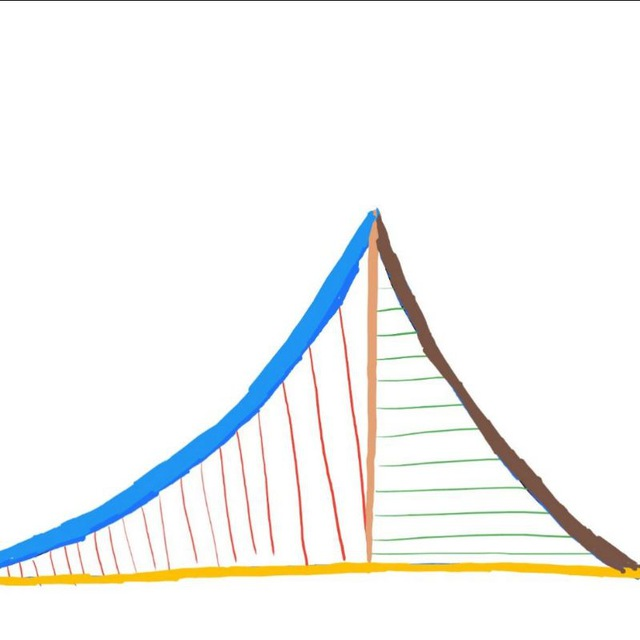
\includegraphics[scale=0.07]{logo.jpg}}\hspace{12.425cm}\raggedleft FWC22025\vspace{2mm}\\
\centering\Large\textbf{MATRICES-CONICS}\vspace{5mm}
\begin{multicols}{2}
\centering \large\textsc{C}\footnotesize\textsc{ONTENTS}\vspace{5mm}\\
\raggedright\large\textbf{1\hspace{1cm}Problem}\hspace{5.2cm}1\vspace{5mm}\\
\raggedright\large\textbf{2\hspace{1cm}Solution}\hspace{5.25cm}1\vspace{5mm}\\
\raggedright\large\textbf{3\hspace{1cm}Construction}\hspace{4.25cm}2\vspace{5mm}\\
\centering \large\textsc{1  P}\footnotesize\textsc{ROBLEM}\vspace{5mm}\\
\raggedright\large
	{
\fi
		Find a point on the curve \begin{align}y=(x-2)^2\end{align} at which a tangent is parallel to the chord joining the points (2,0) and (4,4).
			\\
			\solution 
	\begin{figure}[!ht]
		\centering
 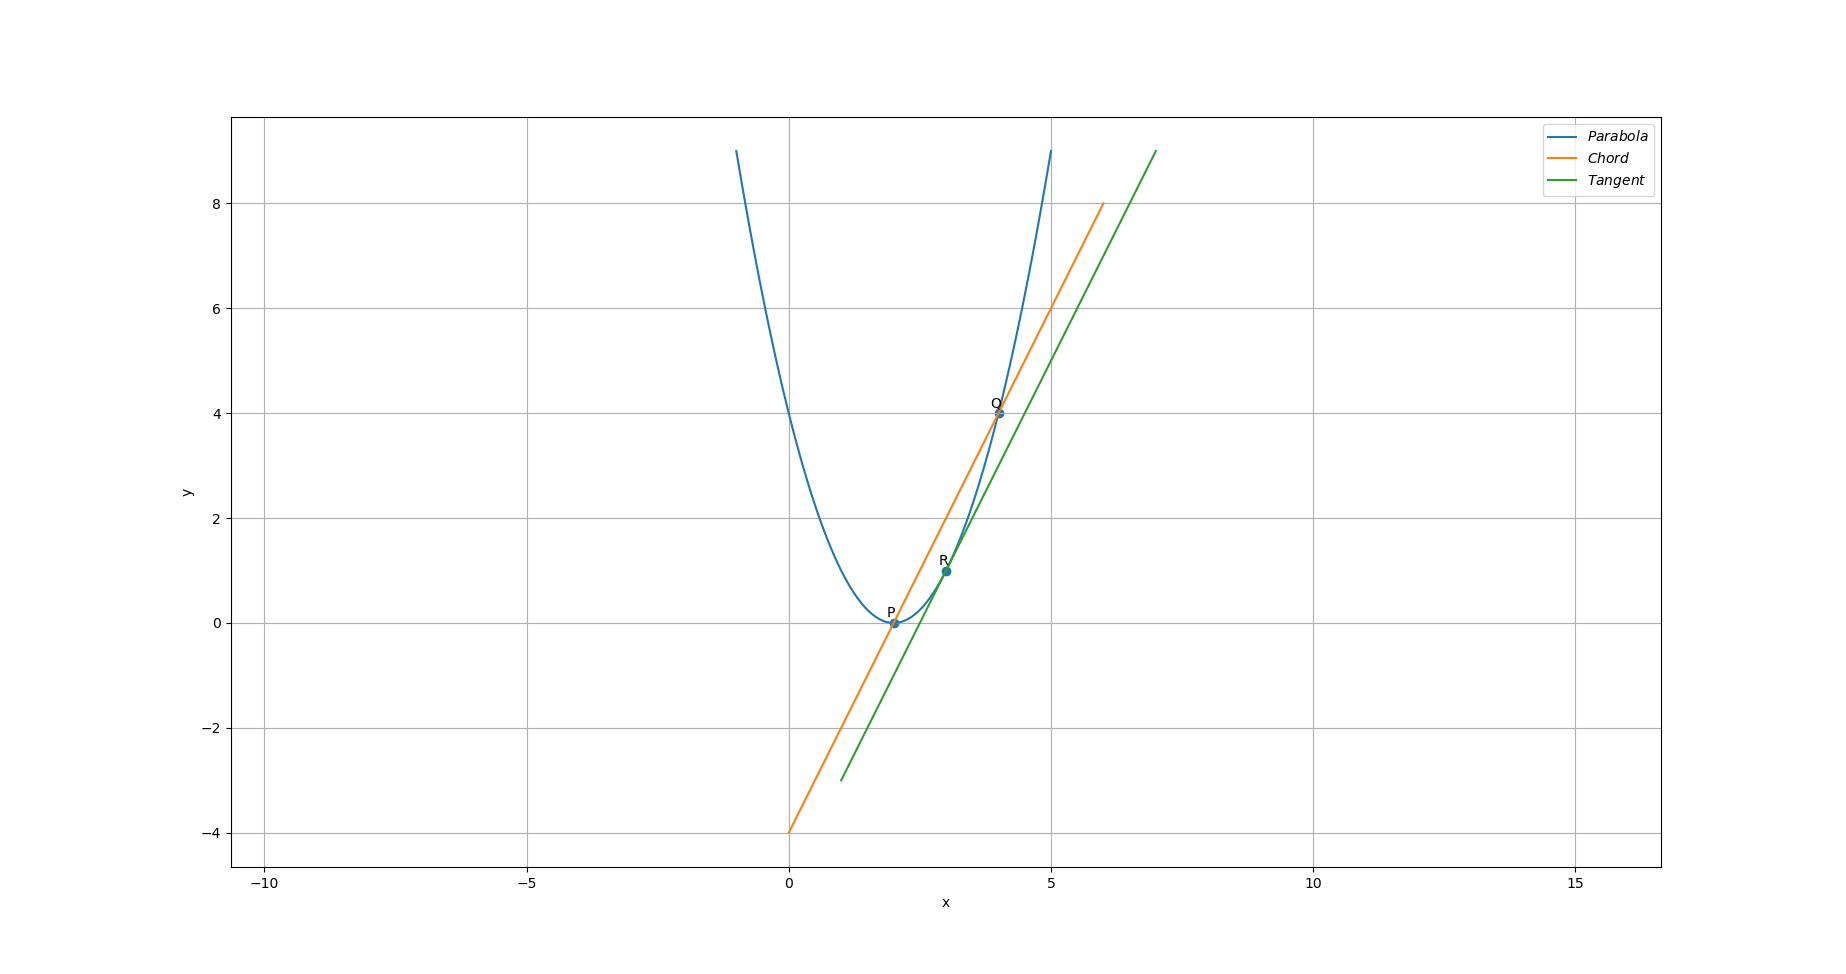
\includegraphics[width=\columnwidth]{chapters/12/6/3/8/figs/main.png}
		\caption{}
		\label{fig:12/6/3/8}
  	\end{figure}
\iffalse
		}\vspace{5mm}\\
\centering \large\textsc{2  S}\footnotesize\textsc{OLUTION}\vspace{5mm}\\
\fi
The equation of the conic can be represented as
\begin{align}
\vec{x}^{\top}\myvec{1&0\\0&0}\vec{x}+2\myvec{-2&\frac{-1}{2}}\vec{x}+4=0
\end{align}
So,
\begin{align}
\vec{V}=\myvec{1&0\\0&0},
\vec{u}^{\top}=\myvec{-2&\frac{-1}{2}},
f=4
\end{align}
The direction vector of the line passing through (2,0) and (4,4) is 
\iffalse
\begin{align*}
\frac{x-2}{1}=\frac{y-0}{2}
\end{align*}
\raggedright\large{So, the direction vector can be given as,}
\fi
\begin{align}
\vec{m}=\myvec{1\\2}
\implies
\vec{n}=\myvec{2\\-1}.
\end{align}
From 
\eqref{eq:conic_tangent_q_eigen},
%Since $\vec{V}$ is not invertible,  given the normal vector $\vec{n}$, 
	the point of contact to parabola is given by 
\begin{align}
		\label{eq:12/6/3/8}
\myvec{
\vec{(u+\kappa \vec{n})}^{\top} \\ \vec{V}
}
\vec{q} &= 
\myvec{
-f
\\
\kappa\vec{n}-\vec{u}
}
\\
\text{where }  \kappa = \frac{\vec{p}_1^{\top}\vec{u}}{\vec{p}_1^{\top}\vec{n}}, \quad \vec{V}\vec{p}_1 &= 0
\end{align}
\iffalse
If $\vec{V}$ is non-invertible, it has a zero eigenvalue.  If the corresponding eigenvector is $\vec{p}_1$, then,
\begin{align}
\vec{V}\vec{p}_1= 0
\end{align}
Let, the eigenvector be 
\begin{align}
\vec{p}_1=\myvec{{x}_1\\{x}_2}\\
\myvec{1&0\\0&0}\myvec{{x}_1\\{x}_2}=0\\
{x}_1=0\\
\vec{p}_1=\myvec{0\\{x}_2}\\
\vec{p}_1=\myvec{0\\1}{x}_2\\
\end{align}
\fi
The eigenvector corresponding to the zero eigenvalue is 
\begin{align}
\vec{p}_1=\myvec{0\\1},
\end{align}
from which, 
%Now, the $\kappa$ can be given as,
\begin{align}
	\kappa&=\frac{\myvec{0&1}\myvec{-2\\ \frac{-1}{2}}}{\myvec{0&1}\myvec{2\\-1}}\\
%\kappa=\frac{\frac{-1}{2}}{-1}\\
	&=\frac{1}{2}
\end{align}
Substituting  $\kappa$ in 
		\eqref{eq:12/6/3/8},
\begin{align}
	\myvec{\sbrak{\myvec{-2\\\frac{-1}{2}}+\frac{1}{2}\myvec{2\\-1}}^{\top} \\ \myvec{1&0\\0&0}}\vec{q} &= \myvec{-4 \\ \frac{1}{2}\myvec{2\\-1}-\myvec{-2\\\frac{-1}{2}}}\\
	\implies
	\myvec{-1&-1 \\ 1&0 \\ 0&0}\vec{q}&=\myvec{-4 \\ 3 \\ 0}
\end{align}
As the last row elements are all zero, we can eliminate that row
\begin{align}
\myvec{-1&-1 \\ 1&0}\vec{q} = \myvec{-4\\3}
\end{align}
For applying row reduction method the augmented matrix is written as
\begin{align}
  \myvec{
                -1&-1&\vrule&-4\\
	        1&0&\vrule&3}\\
  \xleftrightarrow[]{R_1 \leftarrow R_1+ 2R_2}
     \myvec{
	         1&-1&\vrule&2\\
	         1&0&\vrule&3}
      \\
 \xleftrightarrow[]{R_2 \leftarrow R_2 - R_1}
     \myvec{
	         1&-1&\vrule&2\\
	         0&1&\vrule&1}
      \\
 \xleftrightarrow[]{R_1 \leftarrow R_1 + R_2}
     \myvec{
	         1&0&\vrule&3\\
	         0&1&\vrule&1}
      \\ \implies \vec{q}=\myvec{3\\1}
\end{align}
which is the desired 
point of contact.
See Fig. 
		\ref{fig:12/6/3/8}.
\iffalse

\centering{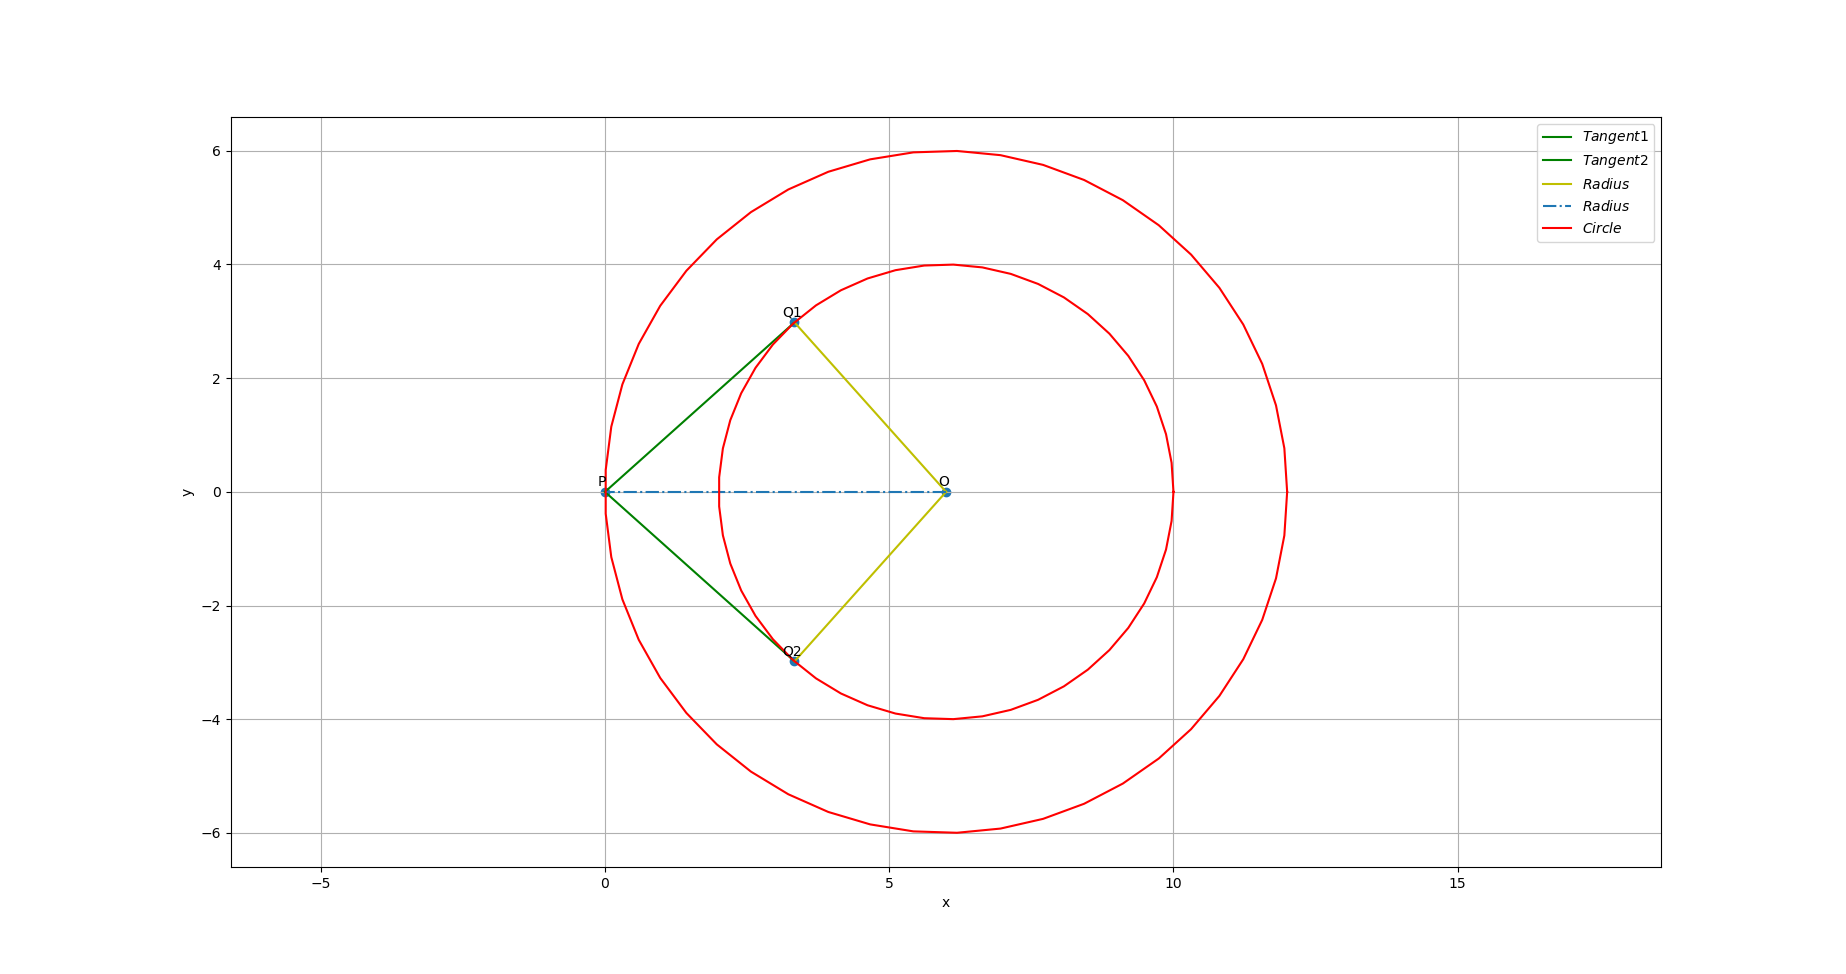
\includegraphics[scale=0.2]{main.png}}\vspace{2mm}\\
\centering{Figure}\vspace{2mm}\\
\centering \large\textsc{3  C}\footnotesize\textsc{ONSTRUCTION}\vspace{5mm}\\
\raggedright\large{The parabola and tangent can be constructed using,} 
\begin{center}
    \label{tab:truthtable}
    \setlength{\arrayrulewidth}{0.2mm}
\setlength{\tabcolsep}{5pt}
\renewcommand{\arraystretch}{1.25}
    \begin{tabular}{|c|c|c|}
    \hline % <-- Alignments: 1st column left, 2nd middle and 3rd right, with vertical lines in between
      \large\textbf{Symbol} & \large\textbf{Co-ordinates} & \large\textbf{Description}\\
      \hline
	\large m & $\ \myvec{ 1\\2 }$ & \large direction vector of PQ\\
       \large P & $\ \myvec{ 2\\0 }$ & \large point vector P\\
	\large Q & $\ \myvec{ 4\\4 }$ & \large point vector Q\\
	\large \textbf{R} & $\vec{q}$ & point of contact\\
      \hline
   \end{tabular}
 \end{center}\vspace{5mm}
\raggedright\large{The figure above is generated using python code provided in the below source code link.}\vspace{2mm}\\
\begin{mdframed}
\raggedright\large{https://github.com/madind5668 \\ /FWC/blob/main/matrices/conics \\ /codes/main.py}
\end{mdframed}
\end{multicols}
\end{document}
\fi
